\chapter{Automi finiti}
La teoria degli automi finiti è nata in relazione a due problematiche completamente diverse.

La prima, in ambiente logico-matematico, riguarda la formalizzazione nel modo più generale possibile della nozione di algoritmo. Contributi fondamentali in questa direzione sono stati dati verso la fine degli anni 30 da ricercatori quali Turing, Church e Kleene.

La seconda ebbe origine verso la metà degli anni 40 ad opera del neurofisiologo McCulloch e del matematico Pitts. Essa riguardava la possibilità di fornire una descrizione matematica del funzionamento delle cellule nervose, o neuroni, e delle reti di neuroni.

\vspace{5mm}

Dai due filoni di ricerca nacquero e si svilupparono due teorie di grande interesse sia per la Matematica che per l’Informatica.
Il primo lavoro che fornisce un’esposizione chiara e abbastanza esauriente della teoria degli automi finiti è un articolo di Rabin e Scott del 1959.

\vspace{5mm}

Esempi di applicazioni di definizioni e risultati della teoria degli automi finiti:
\begin{itemize}
    \item analizzatori lessicali, generatori di analizzatori lessicali
    \item uso delle espressioni regolari in unix/linux
    \item software per trovare occorrenze di parole o frasi in un testo
\end{itemize}
Automi finiti: modello per flip-flop, unità di controllo di un computer, gestione dei processi in un sistema operativo...

Automi finiti: modello per controllo di ascensori, porte scorrevoli, calcolatrici, macchine distributrici di bibite e molti elettrodomestici di uso comune.

\begin{figure}[hbpt!]
    \centering
    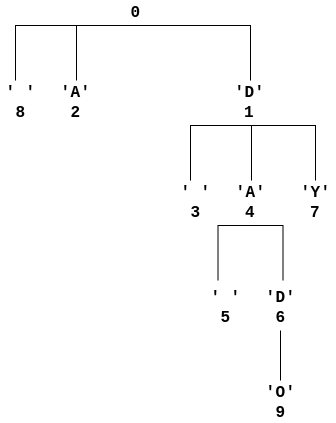
\includegraphics[width=5cm]{./Images/4.1.png}
\end{figure}
\FloatBarrier

I linguaggi associati agli automi finiti (che chiameremo regolari) sono particolarmente utili nella costruzione di compilatori e interpreti nella fase di individuazione dei \textit{token}, cioè degli elementi basilari di un programma, per esempio identificatori, parole chiave, delimitatori, operatori ecc.

Per esempio, il comando seguente
$$
\text { PIPPO : }=3.14+\mathrm{A}
$$
è composto da 18 caratteri e può venir rappresentato ad esempio come la successione di token

$\begin{array}{lllll}1 & 7 & 5 & 2 & 1\end{array}$
in cui si codificano con il token 1 gli identificatori, con il 7 l'operatore di assegnamento, con il 5 una costante, con 2 un operatore aritmetico e con 9 un delimitatore. Naturalmente bisognerà tener traccia del fatto che il primo 1 è associato a PIPPO e il secondo ad A ecc. e questo si fa utilizzando una tabella, detta dei simboli.

\vspace{5mm}

Per verificare la correttezza dal punto di vista strettamente sintattico del comando
$$
\text { PIPPO : }=3.14+\mathrm{A}
$$
per esempio che l'espressione alla destra del := è generabile dalla grammatica delle espressioni aritmetiche, è sufficiente prendere in esame la successione di token
175219

\subsubsection{Il modello mentale}
Un automa finito deterministico è un modello di computazione dotato di una quantità estremamente limitata di memoria. Rappresenta un buon modello di computer.
Possiamo immaginarlo come un sistema che può trovarsi in un numero finito di stati e un “controllo” che si muove da stato a stato in risposta a input esterni.
È dotato di una testina di lettura che può muoversi solo verso destra.
In funzione dello stato in cui si trova e dell’input letto, la macchina cambia stato, poi sposta la testina di lettura sulla cella successiva.
Termina dopo aver letto l’ultimo simbolo sul nastro input; lo stato raggiunto determina se la parola è accettata o no.

\vspace{5mm}

La macchina automa finito incorpora un programma con istruzioni del tipo:
\begin{itemize}
    \item nello stato q se leggi i vai nello stato p
    \item nello stato p se leggi n vai nello stato t
    \item ...
\end{itemize}
Ad ogni passo la testina di lettura si sposta di una cella a destra.
La macchina si ferma quando ha letto tutto l’input.

\subsubsection{Definizione formale di un DFA}
Definizione (Automa a stati finiti deterministico)
Un automa a stati finiti deterministico (in breve DFA) è una quintupla
dove:
$$
\mathcal{A}=\left(Q, \Sigma, \delta, q_{0}, F\right)
$$
\begin{itemize}
    \item Q è l'insieme finito degli stati;
    \item  $\Sigma$ è l'alfabeto (finito);
    \item $q_{0} \in Q$ è lo stato iniziale
    \item $\delta: Q \times \Sigma \rightarrow Q$ è la funzione di transizione;
    \item $F \subseteq Q$ è l'insieme degli stati finali.
\end{itemize}

\subsubsection{Notazioni per DFA}

Specificare un DFA attraverso una quintupla e una descrizione dettagliata della $\delta$ è noioso e di difficile lettura. Sistemi alternativi sono
\begin{itemize}
    \item i diagrammi di stato (o di transizione)
    \item le tabelle di transizione, cioè specifiche tabellari della funzione $\delta$ da cui si deducono l'insieme degli stati e l'alfabeto input. Ovviamente vanno anche specificati stato iniziale e stati finali.
\end{itemize}

Un diagramma di stato per un DFA $\mathcal{A}=\left(Q, \Sigma, \delta, q_{0}, F\right)$ è un grafo orientato definito come segue.
\begin{itemize}
    \item Per ogni stato di $Q$ esiste un nodo.
    \item Per ogni stato $q$ in $Q$ e carattere $a$ in $\Sigma$ se $\delta(q, a)=p$ c'è un arco dal nodo $q$ al nodo $p$ etichettato $a$.
Se $\delta\left(q, a_{1}\right)=\delta\left(q, a_{2}\right)=\ldots=\delta\left(q, a_{n}\right)=p$, il diagramma può avere un solo arco da $q$ a $p$ etichettato $a_{1}, \ldots, a_{n}$.
    \item C'è una freccia entrante nel nodo associato allo stato iniziale $q_{0}$ e tale freccia non proviene da nessun nodo.
    \item I nodi corrispondenti a stati finali sono indicati da un doppio circolo, gli altri da un solo circolo.
    
\end{itemize}

Esempio. Sia $\mathcal{A}=\left(Q, \Sigma, \delta, q_{0}, F\right)$ dove
$$
\begin{aligned}
Q &=\left\{q_{0}, q_{1}, q_{2}\right\} \\
\Sigma &=\{a, b\} \\
F &=\left\{q_{2}\right\} \\
\delta\left(q_{0}, a\right) &=q_{1}, \delta\left(q_{1}, a\right)=q_{1}, \\
\delta\left(q_{1}, b\right) &=q_{2}, \delta\left(q_{2}, b\right)=q_{2}
\end{aligned}
$$

Nota. Non sono definiti né $\delta\left(q_{0}, b\right)$ né $\delta\left(q_{2}, a\right)$ : bisognerebbe aggiungere uno stato "pozzo" come loro risultato, da cui non si esce mai, per nessun simbolo.

\begin{figure}[hbpt!]
    \centering
    \includegraphics[width=6cm]{./Images/4.2.png}
\end{figure}
\FloatBarrier

\subsubsection{Funzione di transizione estesa di un DFA}

Sia $\mathcal{A}=\left(Q, \Sigma, \delta, q_{0}, F\right)$ un automa finito deterministico. La funzione di transizione estesa $\hat{\delta}: Q \times \Sigma^{*} \rightarrow Q$ è definita ricorsivamente come segue
$$
\begin{aligned}
\text { Passo Base } & \forall q \in Q, \\
\hat{\delta}(q, \epsilon) &=q \\
\text { Passo Ricorsivo } & \forall q \in Q, w \in \Sigma^{*}, a \in \Sigma, \\
\hat{\delta}(q, w a) &=\delta(\hat{\delta}(q, w), a)
\end{aligned}
$$

\subsubsection{Linguaggio accettato da un DFA}

Sia $\mathcal{A}=\left(Q, \Sigma, \delta, q_{0}, F\right)$ un automa finito deterministico. II linguaggio accettato o riconosciuto da $\mathcal{A}$ è
$$
L(\mathcal{A})=\left\{w \in \Sigma^{*} \mid \hat{\delta}\left(q_{0}, w\right) \in F\right\}
$$

\begin{figure}[hbpt!]
    \centering
    \includegraphics[width=7cm]{./Images/4.2.png}
\end{figure}
\FloatBarrier

\begin{figure}[hbpt!]
    \centering
    \includegraphics[width=7cm]{./Images/4.3.png}
\end{figure}
\FloatBarrier
\begin{figure}[hbpt!]
    \centering
    \includegraphics[width=7cm]{./Images/4.4.png}
\end{figure}
\FloatBarrier
\begin{figure}[hbpt!]
    \centering
    \includegraphics[width=7cm]{./Images/4.5.png}
\end{figure}
\FloatBarrier
\begin{figure}[hbpt!]
    \centering
    \includegraphics[width=7cm]{./Images/4.6.png}
\end{figure}
\FloatBarrier
\begin{figure}[hbpt!]
    \centering
    \includegraphics[width=7cm]{./Images/4.7.png}
\end{figure}
\FloatBarrier
\begin{figure}[hbpt!]
    \centering
    \includegraphics[width=7cm]{./Images/4.8.png}
\end{figure}
\FloatBarrier
\begin{figure}[hbpt!]
    \centering
    \includegraphics[width=7cm]{./Images/4.9.png}
\end{figure}
\FloatBarrier
\begin{figure}[hbpt!]
    \centering
    \includegraphics[width=8cm]{./Images/4.10.png}
\end{figure}
\FloatBarrier

\subsubsection{Linguaggi regolari}
Un linguaggio $L \subseteq \Sigma^{*}$ è regolare se esiste un DFA $\mathcal{A}$ tale che $L$ è il linguaggio riconosciuto da $\mathcal{A}$, cioè $L=L(\mathcal{A})$.

\subsubsection{Chiusura rispetto a un'operazione}
Una classe di oggetti è chiusa rispetto a un'operazione se
l'applicazione di questa operazione a elementi della classe
restituisce un oggetto ancora nella classe.

\subsubsection{Chiusura rispetto alle operazioni booleane}
Teorema

La classe dei linguaggi regolari è chiusa rispetto al complemento.

Prova (Cenni) 

Sia L un linguaggio regolare, sia $\mathcal{A}=\left(Q, \Sigma, \delta, q_{0}, F\right)$ un DFA che riconosce $L$, cioè $L=L(\mathcal{A})$. Consideriamo il DFA $\mathcal{B}=\left(Q, \Sigma, \delta, q_{0}, Q \backslash F\right)$. II linguaggio riconosciuto da $\mathcal{B}$ è il complemento $\bar{L}$ di $L$. Quindi il complemento $\bar{L}$ di $L$ è regolare.

\vspace{5mm}

Teorema

La classe dei linguaggi regolari è chiusa rispetto a unione e intersezione.
Prova (Cenni) Sia $X$ un linguaggio regolare, sia
$\mathcal{A}_{1}=\left(Q_{1}, \Sigma, \delta_{1}, q_{1}, F_{1}\right)$ un DFA che riconosce $X$, cioè $X=L(\mathcal{A})$.
Sia $Y$ un linguaggio regolare, sia $\mathcal{A}_{2}=\left(Q_{2}, \Sigma, \delta_{2}, q_{2}, F_{2}\right)$ un DFA che riconosce $Y$, cioè $Y=L\left(\mathcal{A}_{2}\right)$.
II DFA $\mathcal{A}=\left(Q_{1} \times Q_{2}, \Sigma, \delta,\left(q_{1}, q_{2}\right), F\right)$, dove $\delta$ è definita come segue:
$$
\begin{gathered}
\forall r_{1} \in Q_{1}, r_{2} \in Q_{2}, a \in \Sigma \\
\delta\left(\left(r_{1}, r_{2}\right), a\right)=\left(\delta_{1}\left(r_{1}, a\right), \delta_{2}\left(r_{2}, a\right)\right)
\end{gathered}
$$
\begin{itemize}
    \item riconosce $X \cap Y$ se $F=F_{1} \times F_{2}$ (e quindi $X \cap Y$ è regolare)
    \item riconosce $X \cup Y$ se $F=\left(Q_{1} \times F_{2}\right) \cup\left(F_{1} \times Q_{2}\right)$ (e quindi $X \cup Y$ è regolare).

\end{itemize}

\begin{figure}[hbpt!]
    \centering
    \includegraphics[width=8cm]{./Images/4.11.png}
\end{figure}
\FloatBarrier

\subsubsection{Automi finiti non deterministici}

Alle volte può essere comodo considerare automi in cui ci siano
alcune transizioni che da certi stati portano con lo stesso simbolo
in più di uno stato.

Infatti è più facile definire in questo modo l'automa per il
linguaggio di interesse e la definizione è spesso più concisa.

Definiamo quindi gli automi a stati finiti non deterministici.
Proveremo che tale estensione non modifica la classe dei linguaggi
riconosciuti.

Vedremo un algoritmo per ottenere un automa deterministico da
uno non deterministico.

Ricordiamo che, dato un insieme X, l'insieme P(X) è l'insieme
potenza di X, ovvero la collezione di tutti i sottoinsiemi di X.

\subsubsection{Definizione formale di un NFA}

Un automa a stati finiti non deterministico (in breve NFA) è una quintupla dove:
$$
\mathcal{A}=\left(Q, \Sigma, \delta, q_{0}, F\right)
$$
\begin{itemize}
    \item  Q è l'insieme finito degli stati;
    \item I è l'alfabeto (finito);
    \item $q_{0} \in Q$ è lo stato iniziale
    \item $\delta: Q \times \Sigma_{\epsilon} \rightarrow \mathcal{P}(Q)$ è la funzione |di transizione, $\operatorname{con} \Sigma_{\epsilon}=\Sigma \cup\{\epsilon\}$
    \item $F \subseteq Q$ è l'insieme degli stati finali.
\end{itemize}
Useremo per rappresentare un NFA le stesse convenzioni adottate
per i DFA.
Nel diagramma di stato vi può essere più di un arco con la stessa
etichetta che porta da uno stato ad altri.

\begin{figure}[hbpt!]
    \centering
    \includegraphics[width=7cm]{./Images/4.12.png}
\end{figure}
\FloatBarrier

\begin{figure}[hbpt!]
    \centering
    \includegraphics[width=8cm]{./Images/4.13.png}
\end{figure}
\FloatBarrier

\begin{figure}[hbpt!]
    \centering
    \includegraphics[width=8cm]{./Images/4.14.png}
\end{figure}
\FloatBarrier

\begin{figure}[hbpt!]
    \centering
    \includegraphics[width=8cm]{./Images/4.15.png}
\end{figure}
\FloatBarrier

\begin{figure}[hbpt!]
    \centering
    \includegraphics[width=8cm]{./Images/4.16.png}
\end{figure}
\FloatBarrier

\subsubsection{$\epsilon$-chiusura}
Definizione
Sia $\mathcal{A}=\left(Q, \Sigma, \delta, q_{0}, F\right)$ un automa finito non deterministico, sia $q \in Q .$ La $\epsilon$-chiusura $E(q)$ di $q$ è un sottoinsieme di $Q$ definito ricorsivamente come segue
$$
\begin{aligned}
\text { Passo Base } & q \in E(q) \\
\text { Passo Ricorsivo } & \forall p \in E(q), \quad \delta(p, \epsilon) \subseteq E(q)
\end{aligned}
$$
Sia $R \subseteq Q$. La $\epsilon$-chiusura $E(R)$ di $R$ è
$$
E(R)=\cup_{q \in R} E(q)
$$

\subsubsection{Funzione di transizione estesa di un NFA}

Sia $\mathcal{A}=\left(Q, \Sigma, \delta, q_{0}, F\right)$ un automa finito non deterministico. La funzione di transizione estesa $\hat{\delta}: Q \times \Sigma^{*} \rightarrow \mathcal{P}(Q)$ è definita ricorsivamente come segue
$$
\begin{aligned}
\text { Passo Base } & \forall q \in Q, \\
\hat{\delta}(q, \epsilon)=& E(q) \\
\text { Passo Ricorsivo } & \forall q \in Q, w \in \Sigma^{*}, a \in \Sigma, \\
\hat{\delta}(q, w a)=& E\left(\cup_{p \in \hat{\delta}(q, w)} \delta(p, a)\right) \\
=& \cup_{p \in \hat{\delta}(q, w)} E(\delta(p, a))
\end{aligned}
$$

\subsubsection{Linguaggio accettato da un NFA}
Sia $\mathcal{A}=\left(Q, \Sigma, \delta, q_{0}, F\right)$ un automa finito non deterministico. 

II linguaggio accettato o riconosciuto da $\mathcal{A}$ è
$$
L(\mathcal{A})=\left\{w \in \Sigma^{*} \mid \hat{\delta}\left(q_{0}, w\right) \cap F \neq \emptyset\right\}
$$

\subsubsection{Equivalenza DFA e NFA}

Teorema

Per ogni automa finito non deterministico $\mathcal{A}$ esiste un automa finito deterministico $\mathcal{B}$ tale che $L(\mathcal{A})=L(\mathcal{B})$.

Prova (Cenni) 

Sia $\mathcal{A}=\left(Q, \Sigma, \delta, q_{0}, F\right)$ un NFA che riconosce $L$, cioè $L=L(\mathcal{A})$. Costruiamo un DFA $\mathcal{B}=\left(Q^{\prime}, \Sigma, \delta^{\prime}, q_{0}^{\prime}, F^{\prime}\right)$ tale che $L(\mathcal{A})=L(\mathcal{B})$
\begin{enumerate}
    \item $Q^{\prime}=\mathcal{P}(Q)$.
Ogni stato di $\mathcal{B}$ è un insieme di stati di $\mathcal{A} .$
    \item $\forall R \in Q^{\prime}, a \in \Sigma$
$$
\delta^{\prime}(R, a)=\cup_{r \in R} E(\delta(r, a))=E\left(\cup_{r \in R} \delta(r, a)\right)
$$
    \item $q_{0}^{\prime}=E\left(\left\{q_{0}\right\}\right)$
    \item $F^{\prime}=\left\{R \in Q^{\prime} \mid R \cap F \neq \emptyset\right\}$
\end{enumerate}

\subsubsection{Caso pessimo}

\begin{figure}[hbpt!]
    \centering
    \includegraphics[width=9cm]{./Images/4.17.png}
\end{figure}
\FloatBarrier

Corollario

Un linguaggio è regolare se e solo se esiste un automa finito non
deterministico che lo riconosce.

\subsubsection{Espressioni regolari}

C'è un terzo modo per esprimere i linguaggi regolari, che va sotto
il nome di espressioni regolari. Le espressioni regolari offrono
notevoli vantaggi di scrittura, e possono essere manipolate in base
ad alcune loro proprietà algebriche senza modificare i linguaggi che
rappresentano.


Le espressioni regolari sono un utile strumento nel progetto dei
compilatori per i linguaggi di programmazione. Gli oggetti
elementari in un linguaggio di programmazione, chiamati \textit{token},
come i nomi delle variabili e le costanti, possono essere descritti
con espressioni regolari.

Una volta che la sintassi di un linguaggio di programmazione è
stata descritta usando espressioni regolari per i suoi token, dei
sistemi automatici possono generare l'analizzatore lessicale, la parte
di un compilatore che elabora inizialmente il programma input.

Definizione ricorsiva delle espressioni regolari su un alfabeto $\Sigma:$

\textbf{PASSO BASE:}

Per ogni $a \in \Sigma, a$ è un'espressione regolare;
\begin{itemize}
    \item $\epsilon$ è un'espressione regolare;
    \item $\emptyset$ è un'espressione regolare.
\end{itemize}

\textbf{PASSO RICORSIVO:} 

Se $E_{1}, E_{2}$ sono espressioni regolari, allora
\begin{itemize}
    \item $\left(E_{1}\right)$ è un'espressione regolare;
    \item $\left(E_{1}+E_{2}\right)$ è un'espressione regolare;
    \item $\left(E_{1} E_{2}\right)$ è un'espressione regolare;
    \item $\left(E_{1}^{*}\right)$ è un'espressione regolare.
\end{itemize}

Definizione ricorsiva dei linguaggi rappresentati dalle espressioni regolari su un alfabeto $\Sigma$.

Data un'espressione regolare $E$, indicheremo con $L(E)$ il linguaggio che essa rappresenta, definito come segue

\textbf{PASSO BASE:}

Per ogni $a \in \Sigma, L(a)=\{a\} ;$
\begin{itemize}
    \item $L(\epsilon)=\{\epsilon\} ;$
    \item $L(\emptyset)=\emptyset$.
\end{itemize}


\textbf{PASSO RICORSIVO:}

Se $E_{1}, E_{2}$ sono espressioni regolari, allora
\begin{itemize}
    \item $L\left(\left(E_{1}\right)\right)=L\left(E_{1}\right) ;$
    \item $L\left(E_{1}+E_{2}\right)=L\left(E_{1}\right) \cup L\left(E_{2}\right) ;$
    \item $L\left(E_{1} E_{2}\right)=L\left(E_{1}\right) L\left(E_{2}\right) ;$
    \item $L\left(E_{1}^{*}\right)=L\left(E_{1}\right)^{*} .$
\end{itemize}

\subsubsection{Regole di precedenza degli operatori}
\vspace{5mm}
\begin{center}
    \begin{tabular}{|r|l|}
\hline Operatore & precedenza \\
\hline$*$ & 1 \\
$\cdot$ & 2 \\
$+$ & 3 \\
\hline
\end{tabular}
\end{center}

\vspace{5mm}

L'espressione regolare $a b^{*}+b$ corrisponde $a\left(a(b)^{*}\right)+b$ ed è diversa da $(a b)^{*}+b$.
L'espressione regolare $a b^{*}+b$ è anche diversa da $a\left(b^{*}+b\right)$.

\subsubsection{Teorema di Kleene}

Un linguaggio è regolare se e solo se esiste un'espressione regolare
che lo rappresenta.

Prova (Cenni): dall'espressione regolare all'automa


Supponiamo di avere un'espressione regolare $E$ che descrive un
linguaggio $L$. Mostriamo come trasformare $E$ in un NFA che
riconosce $L$.
È una dimostrazione per induzione strutturale.

PASSO BASE:

Se $E=a$, con $a \in \Sigma$ allora $L(a)=\{a\}$. Risulta $L(E)=L(\mathcal{A})$,
$\mathcal{A}=\left(\left\{q_{1}, q_{2}\right\}, \Sigma, \delta, q_{1},\left\{q_{2}\right\}\right)$, dove $\delta$ è definita da
$\delta\left(q_{1}, a\right)=\left\{q_{2}\right\}$ e $\delta(r, b)=\emptyset$ per $r \neq q_{1} \circ b \neq a ;$

Se $E=\epsilon$, allora $L(\epsilon)=\{\epsilon\} .$ Risulta $L(E)=L(\mathcal{A})$,
$\mathcal{A}=\left(\left\{q_{1}\right\}, \Sigma, \delta, q_{1},\left\{q_{1}\right\}\right)$, dove $\delta(r, b)=\emptyset$ per ogni $r$ e $b ;$

Se $E=\emptyset$, allora $L(\emptyset)=\emptyset$. Risulta $L(E)=L(\mathcal{A})$,
$\mathcal{A}=\left(\left\{q_{1}\right\}, \Sigma, \delta, q_{1}, \emptyset\right)$, dove $\delta(r, b)=\emptyset$ per ogni $r$ e $b .$

\begin{figure}[hbpt!]
    \centering
    \includegraphics[width=3cm]{./Images/4.18.png}
\end{figure}
\FloatBarrier

PASSO INDUTTIVO:

Siano $E_{1}, E_{2}$ espressioni regolari. Allora

$L\left(E_{1}+E_{2}\right)=L\left(E_{1}\right) \cup L\left(E_{2}\right) ;$

$L\left(E_{1} E_{2}\right)=L\left(E_{1}\right) L\left(E_{2}\right) ;$

$L\left(E_{1}^{*}\right)=L\left(E_{1}\right)^{*}$

sono linguaggi regolari.

\vspace{5mm}

Teorema

La classe dei linguaggi regolari è chiusa rispetto a unione,
concatenazione e star.

Prova (Cenni) 

Sia $X$ un linguaggio regolare, sia $\mathcal{A}_{1}=\left(Q_{1}, \Sigma, \delta_{1}, q_{1}, F_{1}\right)$ un NFA che riconosce $X$, cioè $X=L(\mathcal{A})$. Sia $Y$ un linguaggio regolare, sia $\mathcal{A}_{2}=\left(Q_{2}, \Sigma, \delta_{2}, q_{2}, F_{2}\right)$ un NFA che riconosce $Y$, cioè $Y=L\left(\mathcal{A}_{2}\right)$.

\begin{figure}[hbpt!]
    \centering
    \includegraphics[height=4cm]{./Images/4.19.png}
\end{figure}
\FloatBarrier

Costruiamo $\mathcal{A}=\left(Q, \Sigma, \delta, q_{0}, F\right)$ per riconoscere $X \cup Y$.
\begin{enumerate}
    \item $Q=\left\{q_{0}\right\} \cup Q_{1} \cup Q_{2}$.
Gli stati di $\mathcal{A}$ sono tutti gli stati di $\mathcal{A}_{1}$ e $\mathcal{A}_{2}$, con l'aggiunta di un nuovo stato iniziale $q_{0}$.
    \item Lo stato $q_{0}$ è lo stato iniziale di $\mathcal{A}$.
    \item L'insieme degli stati finali $F=F_{1} \cup F_{2}$.
Gli stati accettanti di $\mathcal{A}$ sono tutti gli stati accettanti di $\mathcal{A}_{1}$ e $\mathcal{A}_{2} .$
    \item Definiamo $\delta$ in modo che per ogni $q \in Q$ e ogni $a \in \Sigma_{\epsilon}$,
$$
\delta(q, a)= \begin{cases}\delta_{1}(q, a) & \text { se } q \in Q_{1} \\ \delta_{2}(q, a) & \text { se } q \in Q_{2} \\ \left\{q_{1}, q_{2}\right\} & \text { se } q=q_{0} \text { e } a=\epsilon \\ \emptyset & \text { se } q=q_{0} \text { e } a \neq \epsilon\end{cases}
$$
\end{enumerate}

\begin{figure}[hbpt!]
    \centering
    \includegraphics[width=7cm]{./Images/4.20.png}
\end{figure}
\FloatBarrier

Costruiamo $\mathcal{A}=\left(Q, \Sigma, \delta, q_{1}, F_{2}\right)$ per riconoscere $X \cdot Y$.
\begin{enumerate}
    \item  $Q=Q_{1} \cup Q_{2}$.
Gli stati di $\mathcal{A}$ sono tutti gli stati di $\mathcal{A}_{1}$ e $\mathcal{A}_{2}$.
    \item Lo stato $q_{1}$ è uguale allo stato iniziale di $\mathcal{A}_{1}$.
    \item L'insieme degli stati finali $F_{2}$ di $\mathcal{A}$ è uguale all'insieme degli stati finali di $\mathcal{A}_{2}$.
    \item Definiamo $\delta$ in modo che per ogni $q \in Q$ e ogni $a \in \Sigma_{\epsilon}$,
$$
\delta(q, a)= \begin{cases}\delta_{1}(q, a) & \text { se } q \in Q_{1} \text { e } q \notin F_{1} \\ \delta_{1}(q, a) & \text { se } q \in F_{1} \text { e } a \neq \epsilon \\ \delta_{1}(q, a) \cup\left\{q_{2}\right\} & \text { se } q \in F_{1} \text { e } a=\epsilon \\ \delta_{2}(q, a) & \text { se } q \in Q_{2} .\end{cases}
$$
\end{enumerate}

\begin{figure}[hbpt!]
    \centering
    \includegraphics[width=7cm]{./Images/4.21.png}
\end{figure}
\FloatBarrier

Costruiamo $\mathcal{A}=\left(Q, \Sigma, \delta, q_{0}, F\right)$ per riconoscere $X^{*}$.
\begin{enumerate}
    \item $Q=\left\{q_{0}\right\} \cup Q_{1}$.
Gli stati di $\mathcal{A}$ sono gli stati di $\mathcal{A}_{1}$ più un nuovo stato $q_{0}$.
    \item Lo stato $q_{0}$ è il nuovo stato iniziale.
    \item  $F=\left\{q_{0}\right\} \cup F_{1}$.
    \item  Definiamo $\delta$ in modo che per ogni $q \in Q$ e ogni $a \in \Sigma_{\epsilon}$,
$$
\delta(q, a)= \begin{cases}\delta_{1}(q, a) & \text { se } q \in Q_{1} \text { e } q \notin F_{1} \\ \delta_{1}(q, a) & \text { se } q \in F_{1} \text { e } a \neq \epsilon \\ \delta_{1}(q, a) \cup\left\{q_{1}\right\} & \text { se } q \in F_{1} \text { e } a=\epsilon \\ \left\{q_{1}\right\} & \text { se } q=q_{0} \text { e } a=\epsilon \\ \emptyset & \text { se } q=q_{0} \text { e } a \neq \epsilon\end{cases}
$$
\end{enumerate}

\begin{figure}[hbpt!]
    \centering
    \includegraphics[width=7cm]{./Images/4.22.png}
\end{figure}
\FloatBarrier

\begin{figure}[hbpt!]
    \centering
    \includegraphics[width=8cm]{./Images/4.23.png}
\end{figure}
\FloatBarrier

Esistono almeno due algoritmi per trasformare un DFA in
un'espressione regolare equivalente
\begin{itemize}
    \item Metodo di Kleene
    \item Metodo di Brzozowski e McCluskey (BMC)
\end{itemize}

\subsubsection{Metodo di Kleene}
Supponiamo che $\mathcal{A}=(Q, \Sigma, \delta, 1, F)$ sia un DFA in cui gli stati sono indicati con numeri interi positivi.


Sia $Q=\{1,2, \ldots, n\}, n \geq 1$.

Indichiamo con $R_{i, j}^{(k)}$ il linguaggio delle etichette dei cammini da $i$ a $j$ i cui nodi interni sono minori o uguali a $k$.

$R_{i, j}^{(0)}$ sarà il linguaggio delle etichette dei cammini da $i$ a $j$ che non hanno nodi interni.

Quindi $R_{i, j}^{(0)}$ sarà il linguaggio delle etichette dei cammini da $i$ a $j$ di lunghezza 0 oppure $1 .$

\vspace{5mm}

Inoltre $R_{i, j}^{(n)}$ sarà il linguaggio delle etichette dei cammini da $i$ a $j$.

Infatti ogni stato in $\mathcal{A}$ è rappresentato da un numero minore o uguale a $n$.
Quindi
$$
L(\mathcal{A})=\bigcup_{j \in F} R_{1, j}^{(n)}
$$

È possibile provare che esiste un'espressione regolare, denotata con abuso di notazione ancora con $R_{i, j}^{(k)}$, che rappresenta il linguaggio $R_{i, j}^{(k)}$ delle etichette dei cammini da $i$ a $j$ i cui nodi interni sono minori o uguali a $k$.

Quindi esiste un'espressione regolare che denota $L(\mathcal{A})$ ed è
$$
\sum_{j \in F} R_{1, j}^{(n)}
$$

\begin{figure}[hbpt!]
    \centering
    \includegraphics[width=8cm]{./Images/4.24.png}
\end{figure}
\FloatBarrier

Usando il principio di induzione è possibile provare che esiste un'espressione regolare che denota $R_{i, j}^{(k)}$, per ogni $i, j, k$.

La prova fornisce un algoritmo ricorsivo per calcolare le espressioni $R_{i, j}^{(k)}$ e quindi anche l'espressione regolare che denota $L(\mathcal{A})$.

\vspace{5mm}

Proviamo che esiste un'espressione regolare che denota $R_{i, j}^{(k)}$ per induzione su $k$.

\textbf{PASSO BASE:} $k=0 .$
$$
R_{i, j}^{(0)}= \begin{cases}\sum_{\delta(i, a)=j} a & \text { se } i \neq j \\ \left(\sum_{\delta(i, a)=j} a\right)+\epsilon & \text { se } i=j\end{cases}
$$


\textbf{PASSO INDUTTIVO:} Se esiste un'espressione regolare che denota $R_{t, s}^{(k-1)}$, per ogni $t, s$, allora esiste un'espressione regolare che denota $R_{i, j}^{(k)}$, per ogni $i, j$. Infatti:
$$
R_{i, j}^{(k)}=R_{i, j}^{(k-1)}+R_{i, k}^{(k-1)}\left(R_{k, k}^{(k-1)}\right)^{*} R_{k, j}^{(k-1)}
$$

\begin{figure}[hbpt!]
    \centering
    \includegraphics[width=7cm]{./Images/4.25.png}
\end{figure}
\FloatBarrier

Il metodo BMC consiste nel calcolare, per ogni stato finale $q$, l'espressione regolare corrispondente ai cammini nell'automa dallo stato iniziale a $q$.

L'espressione si ottiene eliminando gli stati intermendi mediante una particolare procedura.

L'espressione regolare equivalente all'automa sarà l'unione delle espressioni precedentemente ottenute.

\section{Automi e grammatiche regolari}
Vogliamo dimostrare che gli automi finiti deterministici sono
la controparte, in termini di automi, delle grammatiche del
livello più basso della gerarchia di Chomsky: le grammatiche
di tipo 3 o regolari.
Faremo riferimento alla definizione estesa di grammatica di
tipo 3.
Quindi il potere computazionale delle grammatiche di tipo 3 è
lo stesso di quello degli automi.
Otteniamo una nuova caratterizzazione dei linguaggi regolari.

\subsubsection{Grammatiche regolari}

Una grammatica $G=(V, T, P, S)$ è una grammatica di tipo 3 o regolare se ogni produzione è della forma $A \rightarrow a B$ o $A \rightarrow a$, dove $A, B$ sono variabili e a è un terminale.

Inoltre, se $S \rightarrow \epsilon$ è una produzione in $P$ allora $S$ non compare alla destra di nessuna produzione in $P$.

\subsubsection{Definizione formale di un DFA}

Un automa a stati finiti deterministico (in breve DFA) è una quintupla dove:
$$
\mathcal{A}=\left(Q, \Sigma, \delta, q_{0}, F\right)
$$
\begin{itemize}
    \item Q è l'insieme finito degli stati;
    \item $\Sigma$ è l'alfabeto (finito);
    \item $q_{0} \in Q$ è lo stato iniziale
    \item $\delta: Q \times \Sigma \rightarrow Q$ è la funzione di transizione;
    \item $F \subseteq Q$ è l'insieme degli stati finali.
\end{itemize}

\subsubsection{Definizione formale di un NFA}

Un automa a stati finiti non deterministico (in breve NFA) è una quintupla dove:
$$
\mathcal{A}=\left(Q, \Sigma, \delta, q_{0}, F\right)
$$
\begin{itemize}
    \item Q è l'insieme finito degli stati;
    \item $\Sigma$ è l'alfabeto (finito);
    \item $q_{0} \in Q$ è lo stato iniziale
    \item $\delta: Q \times \Sigma_{\epsilon} \rightarrow \mathcal{P}(Q)$ è la funzione di transizione, con $\Sigma_{\epsilon}=\Sigma \cup\{\epsilon\}$ e dove $\mathcal{P}(Q)$ è l'insieme potenza di $Q$,
    \item $F \subseteq Q$ è l'insieme degli stati finali.

\end{itemize}

\subsubsection{Grammatiche regolari e automi}
Proveremo le affermazioni seguenti.
\begin{enumerate}
    \item Per ogni automa a stati finiti deterministico $\mathcal{A}$ esiste una grammatica regolare $G$ tale che $L(\mathcal{A})=L(G)$.
    \item Per ogni grammatica regolare $G$ esiste un automa a stati finiti non deterministico $\mathcal{A}$ tale che $L(\mathcal{A})=L(G)$
\end{enumerate}

\subsubsection{Dall'automa alla grammatica}

\begin{figure}[hbpt!]
    \centering
    \includegraphics[width=6cm]{./Images/4.26.png}
\end{figure}
\FloatBarrier

La computazione dell'automa su aabbb
$$
q_{0} \stackrel{a}{\rightarrow} q_{1} \stackrel{a}{\rightarrow} q_{1} \stackrel{b}{\rightarrow} q_{2} \stackrel{b}{\rightarrow} q_{2} \stackrel{b}{\rightarrow} q_{2}
$$
Come potremmo simularla con le derivazioni in una grammatica?
$$
q_{0} \Rightarrow a q_{1} \Rightarrow a a q_{1} \Rightarrow a a b q_{2} \Rightarrow a a b b q_{2} \Rightarrow a a b b b
$$
E quindi quali produzioni?
$$
q_{0} \rightarrow a q_{1}, \quad q_{1} \rightarrow a q_{1}\left|b q_{2}\right| b, \quad q_{2} \rightarrow b q_{2} \mid b
$$

\begin{figure}[hbpt!]
    \centering
    \includegraphics[width=6cm]{./Images/4.27.png}
\end{figure}
\FloatBarrier

Figura: Un DFA che accetta $\{0,1\}^{*} \backslash\left\{w 1 \mid w \in\{0,1\}^{*}\right\}$
$$
\begin{aligned}
q_{1} \rightarrow 0 q_{1}|0| 1 q_{2}, \quad q_{2} \rightarrow 1 q_{2}\left|0 q_{1}\right| 0 & \\
S \rightarrow q_{1} \mid S \rightarrow \epsilon &
\end{aligned}
$$

Teorema

Per ogni automa finito deterministico $\mathcal{A}$ esiste una grammatica regolare $G$ tale che $L(\mathcal{A})=L(G)$.
\begin{itemize}
    \item  La grammatica che simula l'automa avrà come insieme di variabili (un insieme in corrispondenza biunivoca con) |'insieme degli stati di $\mathcal{A}$. Una variabile ausiliaria $S$ è necessaria se $L(\mathcal{A})$ contiene la parola vuota, cioè se $q_{0} \in F$.
    \item A ogni transizione da uno stato a un altro etichettata da un simbolo è associata una produzione se lo stato di arrivo non è finale, due se lo stato è finale.
    \item Il simbolo iniziale sarà lo stato iniziale di $\mathcal{A}$ se $L(\mathcal{A})$ non contiene la parola vuota, sarà $S$ se $L(\mathcal{A})$ contiene la parola vuota. In questo secondo caso, occorre aggiungere due ulteriori produzioni.
\end{itemize}

Prova. 

Sia $\mathcal{A}=\left(Q, \Sigma, \delta, q_{0}, F\right)$ un automa finito deterministico.


Consideriamo una grammatica $G$ definita come segue:
$$
G= \begin{cases}\left(Q, \Sigma, P, q_{0}\right) & \text { se } q_{0} \notin F \\ \left(Q \cup\{S\}, \Sigma, P^{\prime}, S\right) & \text { se } q_{0} \in F\end{cases}
$$
con $S \notin Q$ e $P, P^{\prime}$ definiti come segue
\begin{enumerate}
    \item $B \rightarrow a C$ è in $P$ se $\delta(B, a)=C$
    \item $B \rightarrow a$ è in $P$ se $\delta(B, a)=C$ e $C \in F$
    \item $P^{\prime}=P \cup\left\{S \rightarrow q_{0}, S \rightarrow \epsilon\right\}$
\end{enumerate}

Si può dimostrare che $L(\mathcal{A})=L(G)$.

\begin{figure}[hbpt!]
    \centering
    \includegraphics[width=6cm]{./Images/4.26.png}
\end{figure}
\FloatBarrier

$$
\begin{aligned}
&G=\left(V, T, P, q_{0}\right) \\
&V=\left\{q_{0}, q_{1}, q_{2}\right\} \\
&T=\{a, b\}
\end{aligned}
$$
$P$ contiene le produzioni
$$
q_{0} \rightarrow a q_{1}, \quad q_{1} \rightarrow a q_{1}\left|b q_{2}\right| b, \quad q_{2} \rightarrow b q_{2} \mid b
$$

\begin{figure}[hbpt!]
    \centering
    \includegraphics[width=6cm]{./Images/4.28.png}
\end{figure}

$$
G=(V, T, P, A), \quad V=\{A, B, C, D\}, \quad T=\{a, b\}
$$
$P$ contiene le produzioni
$$
\begin{aligned}
&A \rightarrow a B|b B, \quad B \rightarrow b C| a D \mid a, \\
&C \rightarrow a D|a| b D|b, \quad D \rightarrow a D| a|b D| b
\end{aligned}
$$

\subsubsection{Dalla grammatica all'automa}

\textbf{Esempio 1.} Consideriamo la grammatica regolare $G_{1}=\left(\{S, B, C\},\{0,1\}, P_{1}, S\right)$, dove le produzioni in $P_{1}$ sono:
$$
S \rightarrow 0 S|1 S| 1 B, \quad B \rightarrow 0 C|1 C, \quad C \rightarrow 0| 1
$$

\begin{figure}[hbpt!]
    \centering
    \includegraphics[width=9cm]{./Images/4.29.png}
\end{figure}
\FloatBarrier

Esempio 1. Consideriamo la grammatica regolare
$G_{1}=\left(\{S, B, C\},\{0,1\}, P_{1}, S\right)$, dove le produzioni in $P_{1}$ sono:
$$
S \rightarrow 0 S|1 S| 1 B, \quad B \rightarrow 0 C|1 C, \quad C \rightarrow 0| 1
$$
Esempio 2. $G_{2}=\left(\{S, B, C, D\},\{0,1\}, P_{2}, S\right)$, dove le
produzioni in $P_{2}$ sono:
$S \rightarrow 0 S|1 S| 1 B, \quad B \rightarrow 0 C|1 C, \quad C \rightarrow 0 D| 1 D|0| 1$

100 è generata, 101 è generata.

\vspace{5mm}


Esempio 3. $G_{3}=\left(\{S, B, C, D\},\{0,1, a\}, P_{2}, S\right)$, dove le
produzioni in $P_{3}$ sono:
$S \rightarrow 0 S|1 S| 1 B, B \rightarrow 0 C|1 C, C \rightarrow 0 D| 1 D|0, D \rightarrow a D| a$

100 è generata, 101 non è generata.


\textbf{Teorema}

Per grammatica regolare $G$ esiste un automa non deterministico tale che $L(\mathcal{A})=L(G)$.
\begin{itemize}
    \item L'automa avrà come come insieme degli stati (un insieme in corrispondenza biunivoca con) l'insieme delle variabili di $G$ più uno stato $A$ che sarà uno stato finale.
    \item Se $S \rightarrow \epsilon$ è in $P$, dove $S$ è il simbolo iniziale della grammatica, allora anche $S$ sarà finale. Ricordiamo che in tal caso $S$ non compare a destra di nessuna produzione in $G$.
    \item 
\end{itemize}

\textbf{Prova.} 

Sia $G=(V, \Sigma, P, S)$ una grammatica regolare. Consideriamo un automa finito non deterministico $\mathcal{A}=(Q, \Sigma, \delta, S, F)$ definito come segue:
$$
\begin{gathered}
Q=V \cup\{A\}, \quad A \notin V \\
F= \begin{cases}\{A\} & \text { se } S \rightarrow \epsilon \notin P \\
\{S, A\} & \text { se } S \rightarrow \epsilon \in P\end{cases}
\end{gathered}
$$
e con $\delta$ tale che
\begin{enumerate}
    \item $C \in \delta(B, a)$ se $B \rightarrow a C$ è in $P$,
    \item $A \in \delta(B, a)$ se $B \rightarrow a$ è in $P$
    \item $\delta(A, a)=\emptyset$, per ogni $a \in \Sigma$
\end{enumerate}

Si può dimostrare che $L(\mathcal{A})=L(G)$.

\vspace{5mm}

Esempio. Consideriamo la grammatica regolare $G=(\{S, B\},\{0,1\}, P, S)$, dove le produzioni in $P$ sono:
$$
S \rightarrow O B, \quad B \rightarrow O B|1 S| 0
$$
Un automa finito non deterministico $\mathcal{A}$ tale che $L(\mathcal{A})=L(G)$ è
$$
\mathcal{A}=(\{S, A, B\},\{0,1\}, \delta, S,\{A\})
$$
dove $\delta$ è definita come segue.
In base alla costruzione del teorema abbiamo
$$
B \in \delta(S, 0), \quad B \in \delta(B, 0), \quad S \in \delta(B, 1), \quad A \in \delta(B, 0)
$$
Quindi
$$
\begin{aligned}
\delta(S, 0) &=\{B\}, \quad \delta(S, 1)=\emptyset \\
\delta(B, 0) &=\{B, A\}, \quad \delta(B, 1)=\{S\} \\
\delta(A, 0) &=\delta(A, 1)=\emptyset
\end{aligned}
$$

\subsubsection{Linguaggi regolari}

\textbf{Teorema}

Un linguaggio L è regolare se e solo se esiste una grammatica regolare $G$ che lo genera, cioè tale che $L=L(G)$.

\subsubsection{Automa minimale}

\begin{figure}[hbpt!]
    \centering
    \includegraphics[width=7cm]{./Images/4.30.png}
\end{figure}
\FloatBarrier

Gli stati $\{q_1, q_2\}$ e $\{q_2, q_3\}$ possono essere "raggruppati".

\begin{figure}[hbpt!]
    \centering
    \includegraphics[width=6cm]{./Images/4.31.png}
\end{figure}
\FloatBarrier

Questo automa $\mathcal{A}$ ha il numero minimo di stati (tra tutti gli automi che riconoscono $L(\mathcal{A})$ ).

Per ogni linguaggio regolare $L$ esiste uno speciale DFA che lo riconosce, chiamato l'automa minimale per $L$.
II nome dipende dal fatto che se $L(\mathcal{A})=L$, con $\mathcal{A}$ automa minimale, per ogni automa $\mathcal{B}$ tale che $L(\mathcal{B})=L$,
\begin{itemize}
    \item $\mathcal{B}$ ha più stati di $\mathcal{A}$
\end{itemize}
oppure
\begin{itemize}
    \item $\mathcal{B}$ ha lo stesso numero di stati di $\mathcal{A}$ e allora i due automi $\mathcal{A}$ e $\mathcal{B}$ sono uguali, a meno di una ridenominazione degli stati.
\end{itemize}
In altri termini, per ogni linguaggio regolare $L$ esiste ed è unico l'automa minimale che riconosce $L$.

\vspace{5mm}
\begin{itemize}
    \item È possibile costruire l'automa minimale di un linguaggio
regolare L a partire da un DFA qualsiasi che riconosce L.
    \item È possibile costruire l'automa minimale di un linguaggio
regolare L a partire da L.
    \item Esiste un algoritmo per costruire l'automa minimale di un linguaggio regolare $L$ a partire da un DFA qualsiasi che riconosce $L$.
    \item Questo algoritmo si basa sulla nozione di stati equivalenti.
    \item Sia $\mathcal{A}=\left(Q, \Sigma, \delta, q_{0}, F\right)$ un DFA. Diremo che $q, q^{\prime} \in Q$ sono equivalenti se le stringhe che portano $\mathcal{A}$ da $q$ a uno stato finale sono le stesse che portano $\mathcal{A}$ da $q^{\prime}$ a uno stato finale.
    \item L'algoritmo divide $Q$ in sottonsiemi formati da stati equivalenti, ognuno dei quali rappresenterà uno stato dell'automa minimale.
    \item Ogni stato nell'automa minimale sarà la fusione di tutti gli stati tra loro equivalenti.
    \item È possibile costruire l'automa minimale di un linguaggio regolare $L$ a partire da $L$.
    \item A ogni DFA $\mathcal{A}=\left(Q, \Sigma, \delta, q_{0}, F\right)$ che riconosce $L$ è possibile associare una relazione, questa volta su $\Sigma^{*}$, che "conta" il numero degli stati.
    \item Diremo che due stringhe $x, y$ sono equivalenti se leggendo l'una o l'altra a partire da $q_{0}, \mathcal{A}$ si troverà nello stesso stato.
    \item Se ogni stato è raggiungibile da $q_{0}$, il numero delle classi è uguale al numero degli stati di $\mathcal{A}$ : minimizzare gli stati equivale a minimizzare il numero delle classi.
    \item Definiremo la relazione di equivalenza di Myhill-Nerode associata a $L$ che ha questo numero minimo di classi. II corrispondente automa, che ha come stati le classi, è l'automa minimale.
\end{itemize}

Esistono algoritmi per costruire l'automa minimale di un
linguaggio regolare L a partire da un DFA qualsiasi che
riconosce L. L'algoritmo che descriveremo in generale non funziona se è
applicato a un NFA che riconosce L.

\subsubsection{Descrizione su un esempio dell'algoritmo}

L'idea di fondo è quella di raggruppare in uno stato solo tutti quelli
che si "comportano" nello stesso modo per poterli sostituire con
un unico stato.

Sia $\mathcal{A}=\left(Q, \Sigma, \delta, q_{0}, F\right)$ un DFA.
Per ogni $q \in Q$, sia $L_{q}=\left\{w \in \Sigma^{*} \mid \hat{\delta}(q, w) \in F\right\}$.


Definizione di stati equivalenti.

Siano $p, q \in Q$
$$
p \equiv q \Leftrightarrow L_{p}=L_{q}
$$
In altri termini, $p \equiv q$ se, per ogni $w \in \Sigma^{*}, \hat{\delta}(p, w)$ è uno stato finale se e solo se $\hat{\delta}(q, w)$ è uno stato finale.

Due stati equivalenti sono anche chiamati indistinguibili.

\begin{figure}[hbpt!]
    \centering
    \includegraphics[width=7cm]{./Images/4.32.png}
\end{figure}
\FloatBarrier

$\Pi_{1}=\left\{\left\{q_{0}, q_{1}, q_{2}, q_{4}, q_{6}\right\},\left\{q_{3}, q_{5}, q_{7}\right\}\right\}$

$\Pi_{2}=\left\{\left\{q_{0}\right\},\left\{q_{1}, q_{2}, q_{4}, q_{6}\right\},\left\{q_{3}, q_{5}, q_{7}\right\}\right\}$

$\Pi_{3}=\left\{\left\{q_{0}\right\},\left\{q_{1}, q_{2}\right\},\left\{q_{4}, q_{6}\right\},\left\{q_{3}, q_{5}, q_{7}\right\}\right\}$

\vspace{5mm}

Nuovo insieme di stati con $A$ stato iniziale:
$$
A=\left\{q_{0}\right\} \quad B=\left\{q_{1}, q_{2}\right\} \quad C=\left\{q_{4}, q_{6}\right\} \quad D=\left\{q_{3}, q_{5}, q_{7}\right\}
$$

\begin{figure}[hbpt!]
    \centering
    \includegraphics[width=6cm]{./Images/4.28.png}
\end{figure}
\FloatBarrier

Definiamo $\bar{\delta}(X, \sigma)=Y$, dove $X, Y$ sono nuovi stati e $\sigma$ è un carattere, se $\delta(q, \sigma)=q^{\prime}$ con $q \in X$ e $q^{\prime} \in Y$ (per esempio $\bar{\delta}(B, b)=C$ perchè $\delta\left(q_{1}, b\right)=q_{4}$ e $\left.q_{1} \in B, q_{4} \in C\right)$.

\subsubsection{Descrizione dell'algoritmo}

Descriviamo formalmente l'algoritmo.

Una \textbf{partizione finita} di un insieme $X$ è una collezione $Y_{1}, \ldots, Y_{n}$ di sottoinsiemi di $X$ tale che $Y_{i} \cap Y_{j}=\emptyset$, $1 \leq i \neq j \leq n \mathrm{e} \cup_{i=1}^{n} Y_{i}=X$.

Una \textbf{partizione} di un insieme $X$ è una collezione $\left(Y_{i}\right)_{i \in I}$ di sottoinsiemi di $X$ tale che $Y_{i} \cap Y_{j}=\emptyset$, per $i, j \in I, i \neq j$ e $\cup_{i \in I} Y_{i}=X$.

\subsubsection{Stati equivalenti}

Sia $\mathcal{A}=\left(Q, \Sigma, \delta, q_{0}, F\right)$ un DFA.

Due stati $p, q \in Q$ sono equivalenti se, per ogni $w \in \Sigma^{*}$, $\hat{\delta}(p, w)$ è uno stato finale se e solo se $\hat{\delta}(q, w)$ è uno stato finale.

\vspace{5mm}

Ora descriviamo un algoritmo ricorsivo. Quando questo algoritmo termina, otteniamo una partizione $\Pi=\left\{Q_{1}, \ldots Q_{n}\right\}$ dell'insieme $Q$ degli stati di $\mathcal{A}$ tale che:
\begin{itemize}
    \item Tutti gli stati in $Q_{i}$ sono equivalenti, $i=1, \ldots, n$
    \item Per ogni $i, j, 1 \leq i \neq j \leq n$, se $p \in Q_{i}$ e $q \in Q_{j}$ allora $p$ e $q$ non sono equivalenti.
\end{itemize}
L'algoritmo individua gli stati $p, q$ NON equivalenti, chiamati per questo distinguibili.

\subsubsection{Algoritmo per individuare gli stati distinguibili}
L'algoritmo per individuare gli stati distinguibili in $\mathcal{A}=\left(Q, \Sigma, \delta, q_{0}, F\right)$ è ricorsivo.

\vspace{5mm}

Algoritmo \texttt{Alg}

\textbf{PASSO BASE:} Se $p \in F$ e $q \notin F$, allora $p$ e $q$ sono stati distinguibili.

\textbf{PASSO RICORSIVO:} Siano $p, q$ due stati tali che, per $a \in \Sigma, r=\delta(p, a)$ ed $s=\delta(q, a)$ siano distinguibili. Allora $p$ e $q$ sono stati distinguibili.

Iniziamo ripartendo $Q$ in due sottoinsiemi usando il passo base.

Ricorsivamente, a ciascuno dei sottoinsiemi ottenuti a un passo precedente applichiamo nuovamente \texttt{Alg}. A ogni passo la regola del passo ricorsivo può essere applicata a un numero finito di coppie (I'insieme $Q$ è finito) e un numero finito di volte a ogni coppia (al più $|\Sigma|$ volte).
Se tale applicazione non produce un cambiamento negli insiemi a cui lo abbiamo applicato, l'algoritmo termina.

L'algoritmo termina sempre. (Caso peggiore: tutti gli insiemi della partizione sono singoletti).

\vspace{5mm}

Teorema

L'algoritmo \texttt{Alg} distingue $p$ e q se e solo se esiste $w \in \Sigma^{*}$ tale che $\hat{\delta}(q, w) \in F \quad e \quad  \hat{\delta}(p, w) \notin F$. Quindi l'algoritmo \texttt{Alg} distingue $p e$ $q$ se e solo se $p$ e q non sono equivalenti.

\vspace{5mm}

Teorema

L'algoritmo \texttt{Alg} non distingue $p$ e $q$ se e solo se $p$ e $q$ sono equivalenti.

Quindi la partizione $\Pi=\left\{Q_{1}, \ldots Q_{n}\right\}$ di $Q$ che otteniamo alla fine dell'algoritmo è tale che $p$ e $q$ sono equivalenti se e solo se esiste $i, 1 \leq i \leq n$, tale che $p \in Q_{i}$ e $q \in Q_{i}$.

\begin{figure}[hbpt!]
    \centering
    \includegraphics[width=7cm]{./Images/4.32.png}
\end{figure}
\FloatBarrier

$\Pi_{1}=\left\{\left\{q_{0}, q_{1}, q_{2}, q_{4}, q_{6}\right\},\left\{q_{3}, q_{5}, q_{7}\right\}\right\}$

$\Pi_{2}=\left\{\left\{q_{0}\right\},\left\{q_{1}, q_{2}, q_{4}, q_{6}\right\},\left\{q_{3}, q_{5}, q_{7}\right\}\right\}$

$\Pi_{3}=\left\{\left\{q_{0}\right\},\left\{q_{1}, q_{2}\right\},\left\{q_{4}, q_{6}\right\},\left\{q_{3}, q_{5}, q_{7}\right\}\right\}$

\begin{itemize}
    \item Applicando il passo base:
$$
\Pi_{1}=\left\{\left\{q_{0}, q_{1}, q_{2}, q_{4}, q_{6}\right\},\left\{q_{3}, q_{5}, q_{7}\right\}\right\}
$$
    \item Poiché $\delta\left(q_{0}, a\right)=q_{1}, \delta\left(q_{1}, a\right)=q_{3}=\delta\left(q_{4}, a\right)$, $\delta\left(q_{2}, a\right)=q_{5}=\delta\left(q_{6}, a\right)$
$$
\Pi_{2}=\left\{\left\{q_{0}\right\},\left\{q_{1}, q_{2}, q_{4}, q_{6}\right\},\left\{q_{3}, q_{5}, q_{7}\right\}\right\}
$$
    \item Poiché $\delta\left(q_{1}, b\right)=q_{4}, \delta\left(q_{2}, b\right)=q_{6}, \delta\left(q_{4}, b\right)=q_{7}$, $\delta\left(q_{6}, b\right)=q_{5}$
$$
\Pi_{3}=\left\{\left\{q_{0}\right\},\left\{q_{1}, q_{2}\right\},\left\{q_{4}, q_{6}\right\},\left\{q_{3}, q_{5}, q_{7}\right\}\right\}
$$
\end{itemize}

\subsubsection{Algoritmo per individuare gli stati equivalenti}

Teorema

L'algoritmo \texttt{Alg} distingue $p$ e q se e solo se esiste $w \in \Sigma^{*}$ tale che $\hat{\delta}(q, w) \in F e \hat{\delta}(p, w) \notin F .$

\vspace{5mm}

Prova (cenni).

Supponiamo che esista $w \in \Sigma^{*}$ tale che $\hat{\delta}(q, w) \in F \mathrm{e} \hat{\delta}(p, w) \notin F$. Proviamo per induzione su $|w|$ che l'algoritmo \texttt{Alg} distingue $p$ e $q$.

Se $w=\epsilon$, allora $q \in F, p \notin F$ e il passo base distingue $p$ e $q$.

Sia $w=a_{1} \cdots a_{n}$, con $a_{i} \in \Sigma, i=1, \ldots, n, n>0$.

Siano
$$
q^{\prime}=\delta\left(q, a_{1}\right), \quad p^{\prime}=\delta\left(p, a_{1}\right), \quad w^{\prime}=a_{2} \cdots a_{n} .
$$
È facile vedere che $\hat{\delta}\left(q^{\prime}, w^{\prime}\right) \in F \mathrm{e} \hat{\delta}\left(p^{\prime}, w^{\prime}\right) \notin F$, con $\left|w^{\prime}\right|<n$.

Per ipotesi induttiva $p^{\prime}, q^{\prime}$ sono distinguibili e, in base al passo ricorsivo dell'algoritmo \texttt{Alg}, anche $p$ e $q$ sono distinguibili.

\vspace{5mm}

Viceversa proviamo che se l'algoritmo \texttt{Alg} distingue $p$ e $q$
allora esiste $w \in \Sigma^{*}$ tale che $\hat{\delta}(q, w) \in F$ e $\hat{\delta}(p, w) \notin F$, per
induzione sul numero di iterazioni necessarie a distinguere $p$ e
$q$ (induzione strutturale).

Se l'algoritmo \texttt{Alg} distingue $p$ e $q$ nel passo base, allora solo
uno dei due è in $F$. Quindi $\hat{\delta}(q, \epsilon) \in F$ e $\hat{\delta}(p, \epsilon) \notin F(\circ$ la
relazione vale scambiando i ruoli di $p$ e $q)$ e $p$ e $q$ non sono
equivalenti.

Supponiamo che l'algoritmo \texttt{Alg} distingue $p$ e $q$ dopo $k>1$
iterazioni. Allora esistono a $\in \Sigma, r=\delta(p, a)$ ed $s=\delta(q, a)$
tali che $r, s$ sono distinguibili.

Per ipotesi induttiva, esiste $w \in \Sigma^{*}$ tale che $\hat{\delta}(r, w) \in F$ e
$\hat{\delta}(s, w) \notin F(o l$ a relazione vale scambiando i ruoli di $r$ e $s)$.

È facile vedere che $\hat{\delta}(p, a w) \in F$ e $\hat{\delta}(q, a w) \notin F .$

Questo conclude la prova.

\subsubsection{Relazione}

Abbiamo dato un algoritmo per il calcolo degli stati
equivalenti in un automa.
Non abbiamo ancora definito l'automa minimale associato a
un linguaggio regolare.

\vspace{4mm}

Una relazione (binaria) $R$ su un insieme $S$ è un insieme di coppie di elementi di $S$.

\vspace{4mm}

Equivalentemente, $R \subseteq S \times S$.

\vspace{4mm}

Scriveremo $a R b$ se $(a, b) \in R$.

\subsubsection{Relazione di equivalenza}

Una relazione (binaria) $R$ su un insieme $S$ è
\begin{itemize}
    \item riflessiva se $a R a$, per ogni $a \in S$
    \item simmetrica se $a R b$ implica $b R a$
    \item transitiva se $a R b$ e $b R c$ implica $a R c$
\end{itemize}

$R$ è una relazione di equivalenza se $R$ è riflessiva, simmetrica e transitiva.

A ogni relazione di equivalenza $R$ su $S$ è associata una partizione in un numero (non necessariamente finito) di classi di equivalenza.

Le classi di equivalenza sono disgiunte e la loro unione fornisce come risultato $S$.

Una classe di equivalenza $E$ con rappresentante $x \in S$ è
$$
E=\{y \in S \mid x R y\}
$$
La classe $E$ viene anche denotata $[x]$.

\subsubsection{Stati equivalenti}

Sia $\mathcal{A}=\left(Q, \Sigma, \delta, q_{0}, F\right)$ un DFA.
Per ogni $q \in Q$, sia $L_{q}=\left\{w \in \Sigma^{*} \mid \hat{\delta}(q, w) \in F\right\} .$

\textbf{Definizione di stati equivalenti.} Siano $p, q \in Q$
$$
p \equiv q \Leftrightarrow L_{p}=L_{q}
$$

In altri termini, $p \equiv q$ se, per ogni $w \in \Sigma^{*}, \hat{\delta}(p, w)$ è uno stato finale se e solo se $\hat{\delta}(q, w)$ è uno stato finale.

Due stati equivalenti sono anche chiamati indistinguibili.

La relazione $\equiv$ è una relazione di equivalenza su $Q$.
[q] denoterà la classe di equivalenza di $q$ rispetto $\mathrm{a} \equiv$

\subsubsection{Stati accessibili}

Sia $\mathcal{A}=\left(Q, \Sigma, \delta, q_{0}, F\right)$ un DFA. Sia $q \in Q$.

Uno stato $q$ è accessibile da $q_{0}$ se esiste una stringa $w \in \Sigma^{*}$ tale che $\hat{\delta}\left(q_{0}, w\right)=q$.

Esistono algoritmi per eliminare da $\mathcal{A}$ gli stati non accessibili da $q_{0}$. Se in $\mathcal{A}$ si eliminano gli stati non accessibili da $q_{0}$ si ottiene un automa equivalente ad $\mathcal{A}$.

\subsubsection{Costruzione dell'automa minimale per L}

Sia $\mathcal{A}=\left(Q, \Sigma, \delta, q_{0}, F\right)$ un DFA che riconosce $L$. L'automa minimale per $L$ è
$$
\mathcal{B}=\left(Q_{m}, \Sigma, \delta_{m},\left[q_{0}\right], F_{m}\right)
$$
dove
$$
\begin{aligned}
Q_{m} &=\left\{[q] \mid q \in Q \text { e q è accessibile da } q_{0}\right\} \\
F_{m} &=\{[q] \mid q \in F\} \\
\delta_{m}([q], a) &=[\delta(q, a)], \quad \text { per ogni }[q] \in Q_{m}, a \in \Sigma
\end{aligned}
$$

Nota: la definizione di $\delta_{m}$ è ben posta.
Infatti, per ogni $q, q^{\prime} \in Q, a \in \Sigma$,
$$
q \equiv q^{\prime} \Rightarrow \delta(q, a) \equiv \delta\left(q^{\prime}, a\right) \Rightarrow[\delta(q, a)]=\left[\delta\left(q^{\prime}, a\right)\right]
$$
Nota: per induzione su $|w|$ si può dimostrare che risulta
$$
\hat{\delta}_{m}([q], w)=[\hat{\delta}(q, w)]
$$
per ogni $q \in Q$ e $w \in \Sigma^{*}$.

\vspace{5mm}

Sia $\mathcal{A}=\left(Q, \Sigma, \delta, q_{0}, F\right)$ un DFA che riconosce $L$.
$$
L(\mathcal{B})=L(\mathcal{A})
$$
Infatti:
$$
\begin{aligned}
w \in L(\mathcal{B}) & \Leftrightarrow \hat{\delta}_{m}\left(\left[q_{0}\right], w\right)=\left[\hat{\delta}\left(q_{0}, w\right)\right] \in F_{m} \\
& \Leftrightarrow \hat{\delta}\left(q_{0}, w\right) \in F \Leftrightarrow w \in L(\mathcal{A})
\end{aligned}
$$

Perché $\mathcal{B}$ è l'automa minimale di $L(\mathcal{A})$ ?

Prova di correttezza dell'algoritmo e Teorema di Myhill-Nerode.

\subsubsection{Relazioni di equivalenza}

Sia $R$ una relazione di equivalenza su $S$.

L'indice di $R$ è il numero delle classi di equivalenza di $R$. Può essere infinito.

Se l'indice di $R$ è finito diciamo che $R$ è di indice finito.

Siano $R_{1}, R_{2}$ relazioni di equivalenza su $S$.
$R_{1}$ è un raffinamento di $R_{2}$ se $R_{1} \subseteq R_{2}$, cioè se
$$
\forall x, y \in S \quad x R_{1} y \Rightarrow x R_{2} y
$$
Se $R_{1}$ è un raffinamento di $R_{2}$ allora ogni classe di equivalenza di $R_{2}$ è unione di alcune classi di equivalenza di $R_{1}$. Quindi, se $R_{1}$ ha indice finito, allora $R_{2}$ ha un minor numero di classi.

Infatti, denotiamo con $[x]_{2}$ la classe di $x$ rispetto ad $R_{2}$ e con $[x]_{1}$ la classe di $x$ rispetto ad $R_{1}$.

Per ogni $y \in[x]_{2}$, risulta $[y]_{1} \subseteq[x]_{2}$. Infatti, se $z \in[y]_{1}$ allora $z R_{1} y$ implica $z R_{2} y$. Quindi $z \in[y]_{2}=[x]_{2}$.
Allora $[x]_{2}=\cup_{y \in[x]_{2}}[y]_{1}$.

\vspace{5mm}

\textbf{Esempio.} Sia $E_{n}$ la congruenza modulo $n$ nell'insieme $\mathbb{Z}$ degli interi.

Quindi $x E_{n} y$ significa $x \equiv y(\bmod n)$
(cioè $x-y$ è un multiplo di $n$ ).

$E_{n}$ ha $n$ classi, corrispondenti alle classi dei resti $(\bmod n)$.

Siccome $x \equiv y(\bmod 6)$ implica $x \equiv y(\bmod 3)$, la relazione $E_{6}$ è un raffinamento di $E_{3}$.
$E_{3}$ ha tre classi: $[0],[1],[2] .$
$E_{6}$ ha sei classi: $[0],[1],[2],[3],[4],[5]$.

Ogni classe di equivalenza di $E_{3}$ è unione di due delle classi di equivalenza di $E_{6}$.

\subsubsection{Due relazioni di equivalenza in $\Sigma^*$}

Sia $\mathcal{A}=\left(Q, \Sigma, \delta, q_{0}, F\right)$ un DFA. Siano $x, y \in \Sigma^{*}$.

La relazione $R_{\mathcal{A}}$ è definita da
$$
x R_{\mathcal{A}} y \quad \Leftrightarrow \quad \hat{\delta}\left(q_{0}, x\right)=\hat{\delta}\left(q_{0}, y\right)
$$
$R_{\mathcal{A}}$ è una relazione di equivalenza e l'indice di $R_{\mathcal{A}}$ è al più $|Q|$. Infatti alla classe di $x$ è associato lo stato $\hat{\delta}\left(q_{0}, x\right)$.


Nota. Perché l'indice di $R_{\mathcal{A}}$ è al più $|Q|$ e non è sempre uguale a $|Q|$ ?


Se $q$ è uno stato di $\mathcal{A}$ non raggiungibile da qo, cioè per il quale non esiste alcuna stringa $z$ tale che $\hat{\delta}\left(q_{0}, z\right)=q$, a $q$ non è associata alcuna classe.

\subsubsection{Relazioni di equivalenza invarianti a destra}

Una relazione di equivalenza $R$ su $\Sigma^{*}$ è invariante a destra (rispetto alla concatenazione) se $x R y$ implica $x z R y z$ per ogni $Z \in \sum^{*}$.
$R_{\mathcal{A}}$ è invariante a destra. Supponiamo $x R_{\mathcal{A}} y$ e proviamo che $x Z R_{\mathcal{A}} y z$.
$$
\begin{aligned}
\hat{\delta}\left(q_{0}, x z\right) &=\hat{\delta}\left(\hat{\delta}\left(q_{0}, x\right), z\right) \\
&=\hat{\delta}\left(\hat{\delta}\left(q_{0}, y\right), z\right) \\
&=\hat{\delta}\left(q_{0}, y z\right)
\end{aligned}
$$

\subsubsection{Due relazioni di equivalenza in $\Sigma^*$}

Sia $\mathcal{A}=\left(Q, \Sigma, \delta, q_{0}, F\right)$ un DFA. Siano $x, y \in \Sigma^{*}$.

La relazione $R_{\mathcal{A}}$ è definita da
$$
x R_{\mathcal{A}} y \quad \Leftrightarrow \quad \hat{\delta}\left(q_{0}, x\right)=\hat{\delta}\left(q_{0}, y\right)
$$
$L=L(\mathcal{A})$ è unione di classi della relazione $R_{\mathcal{A}}$.
Sia $x \in L$, proviamo che la classe di $x$ rispetto ad $R_{\mathcal{A}}$ è contenuta in $L$.

Se $x \in L$ allora $\hat{\delta}\left(q_{0}, x\right) \in F$. Se $y$ è nella classe di $x$ rispetto ad $R_{\mathcal{A}}$, allora $y R_{\mathcal{A}} x$. Quindi $\hat{\delta}\left(q_{0}, y\right)=\hat{\delta}\left(q_{0}, x\right) \in$ F e $y \in L$.

In altri termini, siccome $x \in L \Leftrightarrow \hat{\delta}\left(q_{0}, x\right) \in F$ allora $L$ è unione delle classi che corrispondono agli stati finali di $\mathcal{A}$.

Sia $L \subseteq \Sigma^{*}$. Sia $R_{L}$ definita da: $x R_{L} y$ se e solo se
$$
\forall z \in \Sigma^{*} x z \in L \Leftrightarrow y z \in L
$$
$L$ è unione di classi della relazione di Myhill-Nerode $R_{L}$, le classi che corrispondono agli elementi di $L$.

Infatti sia $x \in L$ e supponiamo $x R_{L} y$.

Applicando la definizione con $z=\epsilon$ otteniamo $y \in L$.

\subsubsection{La relazione $R_L$}

Sia $L=L\left(a^{*} b a^{*}\right)$. Allora $x R_{L} y$ se e solo se vale uno dei seguenti casi
\begin{enumerate}
    \item $x$ e $y$ non hanno occorrenze della lettera $b$
    \item $x$ e $y$ hanno una sola occorrenza della lettera $b$
    \item $x$ e $y$ hanno più di una occorrenza della lettera $b$
Abbiamo quindi tre classi di equivalenza di $R_{L}$, che corrispondono ai linguaggi:
$$
a^{*}, \quad a^{*} b a^{*}, \quad a^{*} b a^{*} b(a \cup b)^{*}
$$

\end{enumerate}

Sia $L=L\left(a^{*} b a^{*}\right)$.

Per vedere perché $R_{L}$ ha tre classi di equivalenza che corrispondono ai linguaggi
$$
a^{*}, \quad a^{*} b a^{*}, \quad a^{*} b a^{*} b(a \cup b)^{*}
$$
osserviamo che questi tre linguaggi costituiscono una partizione di $\{a, b\}^{*}$.

Quindi, presa una stringa in $\{a, b\}^{*}$, distinguiamo tre casi: 
\begin{itemize}
    \item  la stringa non ha occorrenze della lettera $b$, quindi è della forma $a^{i}, i \geq 0 ;$
    \item la stringa ha una sola occorrenza della lettera $b$, quindi è della forma $a^{i} b a^{j}, i, j \geq 0 ;$
    \item la stringa ha più di una occorrenza della lettera $b$, quindi è della forma $a^{i} b a^{j} b z^{\prime}$, con $i, j \geq 0, z^{\prime} \in\{a, b\}^{*}$.

\end{itemize}

Ovvero:

\begin{itemize}
    \item Se $x=a^{i}$ e $y=a^{h} b a^{k}, i, h, k \geq 0$, allora $x$ e $y$ non sono equivalenti perché $x \in \notin L$ mentre $y \epsilon \in L$.
    \item Se $x=a^{i}$ e $y=a^{h} b a^{k} b z^{\prime}, i, h, k \geq 0, z^{\prime} \in\{a, b\}^{*}$, allora $x$ e $y$ non sono equivalenti perché $x b \in L$ mentre $y b \notin L$.
    \item Se $x=a^{i}$ e $y=a^{j}, i, j \geq 0$, allora $x$ e $y$ sono equivalenti perché $x z \in L$ se e solo se $z=a^{h} b a^{k}, h, k \geq 0$, e lo stesso è vero per $y$. Cioè $y z \in L$ se e solo se $z$ ha una sola occorrenza della lettera $b$.
\end{itemize}

Un ragionamento analogo si applica negli altri due casi, cioè se $x=a^{i} b a^{j}$ oppure se $x=a^{i} b a^{j} b z^{\prime}, i, j \geq 0, z^{\prime} \in\{a, b\}^{*}$.

\vspace{5mm}

Sia $L \subseteq \Sigma^{*}$, sia $E$ una relazione di equivalenza su $\Sigma^{*}$ invariante a destra e tale che $L$ è unione di alcune classi di equivalenza di $E$. Allora $E$ è un raffinamento di $R_{L}$, la relazione di equivalenza di Myhill-Nerode.

\vspace{5mm}

\textbf{Prova. }Supponiamo $x$ Ey e proviamo $x R_{L} y$.

Siccome $E$ è invariante a destra e $x E y$, allora per ogni $z$ abbiamo $x z E y z$.

Siccome $L$ è unione di classi di $E$, otteniamo
$$
x z \in L \Leftrightarrow y z \in L
$$
cioè $x R_{L} y$.

\subsubsection{Teorema di Myhill-Nerode}

Le seguenti affermazioni sono equivalenti

\begin{enumerate}[(a)]
 \item $L \subseteq \Sigma^{*}$ è regolare.
 \item L è unione di classi di equivalenza di $E$, dove $E$ è una relazione di equivalenza invariante a destra di indice finito.
 \item $R_{L}$ ha indice finito.
 \end{enumerate}
 
\textbf{Prova (cenni).}

\vspace{5mm}

$(a) \Rightarrow(b) .$ Dobbiamo dimostrare che se $L \subseteq \Sigma^{*}$ è regolare allora $L$ è unione di classi di equivalenza di $E$, dove $E$ è una relazione di equivalenza invariante a destra di indice finito.

Se $L$ è regolare, esiste un DFA $\mathcal{A}$ tale che $L=L(\mathcal{A}) . L$ è unione di classi della relazione $R_{\mathcal{A}}$ ed $R_{\mathcal{A}}$ è una relazione di equivalenza invariante a destra di indice finito.

\vspace{5mm}

$(b) \Rightarrow(c)$. Dobbiamo dimostrare che se $L$ è unione di classi di equivalenza di $E$, dove $E$ è una relazione di equivalenza invariante a destra di indice finito allora $R_{L}$ ha indice finito.

Ma abbiamo dimostrato che ogni relazione di equivalenza $E$ invariante a destra, di indice finito e tale che $L$ è unione di alcune classi di equivalenza di $E$ è un raffinamento di $R_{L}$.

Quindi $E$ è un raffinamento di $R_{L}$. Di conseguenza l'indice di $R_{L}$ è minore o uguale dell'indice di $E$. Siccome $E$ ha indice finito, anche $R_{L}$ ha indice finito.

\vspace{5mm}

(c) $\Rightarrow$ (a). Dobbiamo dimostrare che se $R_{L}$ ha indice finito allora $L$ è regolare.

Denotiamo $[x]$ la classe di $x$ rispetto all'equivalenza $R_{L}$.
Sia $M^{\prime}=\left(Q^{\prime}, \Sigma, \delta^{\prime}, q_{0}^{\prime}, F^{\prime}\right)$ dove
$$
\begin{aligned}
Q^{\prime} &=\left\{[x] \mid x \in \Sigma^{*}\right\} \\
q_{0}^{\prime} &=[\epsilon] \\
F^{\prime} &=\{[x] \mid x \in L\} \\
\delta^{\prime}([x], a) &=[x a], \quad \text { per ogni }[x] \in Q^{\prime}, a \in \Sigma .
\end{aligned}
$$
$Q^{\prime}$ è un insieme finito e vogliamo concludere che $M^{\prime}$ è un DFA che riconosce $L$.

Dobbiamo prima provare che la definizione di $\delta^{\prime}$ è ben posta, cioè che la definizione di $\delta^{\prime}$ non dipende dal rappresentante scelto.

Quindi, siano $x, y \in \Sigma^{*}$ con $y \in[x]$, cioè $[x]=[y]$. Dobbiamo provare che $\delta^{\prime}([x], a)=[x a]=[y a]=\delta^{\prime}([y], a)$.
Per ogni $z \in \Sigma^{*}$,
$$
(x a) z \in L \Leftrightarrow x(a z) \in L \Leftrightarrow y(a z) \in L \Leftrightarrow(y a) z \in L
$$
Quindi $x a R_{L}$ ya cioè $[x a]=[y a]$.

Infine, per induzione su $|y|$ si può provare che $\hat{\delta}([\epsilon], y)=[y]$, per ogni $y \in \Sigma^{*}$.

Da questo segue $L\left(M^{\prime}\right)=L$. (Ricorda che $L$ è unione di classi della relazione $R_{L .}$ )

L'automa $M^{\prime}$ della prova, costruito con le classi di equivalenza di $R_{L}$, è l'automa minimale di $L$.

\vspace{5mm}

\textbf{Teorema}

L'automa $M^{\prime}=\left(Q^{\prime}, \Sigma, \delta^{\prime}, q_{0}^{\prime}, F^{\prime}\right)$ è l'unico automa minimale per $L$, a meno di una ridenominazione degli stati.

\vspace{5mm}

\textbf{Prova (cenni).} Se $M=\left(Q, \Sigma, \delta, q_{0}, F\right)$ è un qualsiasi automa che riconosce $L$, allora $R_{M}$ è un raffinamento di $R_{L}$. Sappiamo che l'indice di $R_{M}$ è al più $|Q|$. Quindi
$$
|Q| \geq \text { indice di } R_{M} \geq \text { indice di } R_{L}=\left|Q^{\prime}\right|
$$
Ogni DFA che riconosce $L$ ha un numero di stati maggiore o uguale al numero degli stati di $M^{\prime}$.

Supponiamo che $M$ ed $M^{\prime}$ abbiano lo stesso numero di stati. Allora le precedenti diseguaglianze diventano uguaglianze:
$$
|Q|=\text { indice di } R_{M}=\text { indice di } R_{L}=\left|Q^{\prime}\right|
$$
Ogni stato $q \in Q$ di $M$ è accessibile da $q_{0}$.
Sia $x$ una stringa tale che $\hat{\delta}\left(q_{0}, x\right)=q$. Identificando $q$ ed $[x]$ otteniamo l'isomorfismo tra $M$ ed $M^{\prime}$.

\subsubsection{Esempio 1}

\textbf{Esempio.} Sia $L=L\left(a^{*} b a^{*}\right)$.
Abbiamo tre classi di equivalenza di $R_{L}$, che corrispondono ai linguaggi $a^{*}, a^{*} b a^{*}, a^{*} b a^{*} b(a \cup b)^{*}:$
$$
q_{0}^{\prime}=[\epsilon], \quad q_{1}^{\prime}=[b], \quad q_{2}^{\prime}=[b b]
$$
L'automa minimale di $L$ è $M^{\prime}=\left(Q^{\prime}, \Sigma, \delta^{\prime}, q_{0}^{\prime}, F^{\prime}\right)$, dove
$$
\begin{aligned}
Q^{\prime} &=\left\{q_{0}^{\prime}, q_{1}^{\prime}, q_{2}^{\prime}\right\} \\
F^{\prime} &=\left\{q_{1}^{\prime}\right\} \\
\delta^{\prime}\left(q_{0}^{\prime}, a\right) &=q_{0}^{\prime}, \quad \delta^{\prime}\left(q_{0}^{\prime}, b\right)=q_{1}^{\prime} \\
\delta^{\prime}\left(q_{1}^{\prime}, a\right) &=q_{1}^{\prime}, \quad \delta^{\prime}\left(\mid q_{1}^{\prime}, b\right)=q_{2}^{\prime} \\
\delta^{\prime}\left(q_{2}^{\prime}, a\right) &=q_{2}^{\prime}, \quad \delta^{\prime}\left(q_{2}^{\prime}, b\right)=q_{2}^{\prime}
\end{aligned}
$$
\clearpage


\subsubsection{Esempio 2}

\begin{figure}[hbpt!]
    \centering
    \includegraphics[width=8cm]{./Images/4.32.png}
\end{figure}
\FloatBarrier

L'automa $M$ riconosce il linguaggio
$L=\left\{a a w, a b a w, a b b w, b a w, b b a w, b b b w \mid w \in\{a, b\}^{*}\right\} .$
La relazione $R_{M}$ è poco interessante: tutti gli stati, tranne quelli finali, definiscono classi con poche parole.

Consideriamo il linguaggio
$L=\left\{a a w, a b a w, a b b w, b a w, b b a w, b b b w \mid w \in\{a, b\}^{*}\right\} .$
Costruiamo le classi di $R_{L}$.

Tutte le stringhe in $L$ formano una sola classe: se $x, y \in L$, per ogni $z$ risulta $x z, y z \in L$. Poniamo $[a a]=D$.

\vspace{5mm}

$L=\left\{\right.$ aaw, abaw, abbw, baw, bbaw, bbbw $\left.\mid w \in\{a, b\}^{*}\right\}$ Consideriamo le altre stringhe:
$$
\{a, b\}^{*} \backslash L=\{\epsilon, a, b, a b, b b\}=L^{\prime}
$$
$\epsilon$ non è equivalente alle altre quattro: $\epsilon a \notin L$ ma ya $\in L$ per $y \in L^{\prime}, y \neq \epsilon$. Poniamo $[\epsilon]=A$.

\vspace{5mm}

$$
\begin{gathered}
L=\left\{a a w, a b a w, a b b w, b a w, b b a w, b b b w \mid w \in\{a, b\}^{*}\right\} . \\
\{a, b\}^{*} \backslash L=\{\epsilon, a, b, a b, b b\}=L^{\prime}
\end{gathered}
$$
Le stringhe $a, b$ formano una classe. Infatti $a, b$ non sono equivalenti ad $a b$ né $a$ bb.

La lettera $b$ "separa" $a$ e $b$ da $a b$ e $b b: a b \notin L, b b \notin L$ mentre $a b b \in L, b b b \in L$.

Inoltre $a$ e $b$ sono equivalenti. Infatti $a z \in L$ se e solo se $z \in\left\{a w, b a w, b b w \mid w \in\{a, b\}^{*}\right\}$ e lo stesso accade per $b z .$ Cioè $b z \in L$ se e solo se $z \in\left\{a w, b a w, b b w \mid w \in\{a, b\}^{*}\right\}$.
Poniamo $[a]=B$.

\vspace{5mm}

$L=\left\{\right.$ aaw, abaw, abbw, baw, bbaw, bbbw $\left.\mid w \in\{a, b\}^{*}\right\} .$
$$
\{a, b\}^{*} \backslash L=\{\epsilon, a, b, a b, b b\}=L^{\prime}
$$
Infine le stringhe $a b, b b$ formano un'altra classe: $a b z \in L$ se e solo se $z \in\left\{a w, b w \mid w \in\{a, b\}^{*}\right\}$ e lo stesso accade per $b b z \in L$. Cioè $b b z \in L$ se e solo se $z \in\left\{a w, b w \mid w \in\{a, b\}^{*}\right\}$. Poniamo $[a b]=C$.

\vspace{5mm}

In conclusione le classi di $R_{L}$ sono quattro:
$$
[\epsilon]=A, \quad[a]=B, \quad[a b]=C, \quad[a a]=D
$$
L'automa minimale $M^{\prime}$ ha quattro stati $A, B, C, D$, stato iniziale $A$, stato finale $D$.

Definendo le transizioni come nella prova del teorema di Myhill-Nerode otteniamo l'automa minimale costruito mediante l'algoritmo \texttt{Alg}.

\begin{figure}[hbpt!]
    \centering
    \includegraphics[width=6cm]{./Images/4.28.png}
\end{figure}
\FloatBarrier

\subsubsection{Costruzione dell'automa minimale per L}

Perché l'automa $M$ per $L$ ottenuto mediante $\mathcal{A} / g$ è (a meno di una ridenominazione degli stati) lo stesso automa $M^{\prime}$ costruito mediante $R_{L}$ ?

Se non lo fosse, ci sarebbero due classi di $R_{M}$, individuate da due stati $p, q$ di $R_{M}$, contenute in una sola classe di $R_{L}$.
Quindi, le etichette dei cammini da $q_{0}$ a $p$ in $M$ e quelle dei cammini da $q_{0}$ a $q$ sarebbero stringhe equivalenti rispetto ad $R_{L}$.

Quindi, per ogni stringa $z$, avremmo che $z$ è etichetta di un cammino da $p$ a uno stato finale se e solo se $z$ è etichetta di un cammino da $q$ a uno stato finale.

Gli stati $p$ e $q$ sarebbero equivalenti ma questo non è possibile nell'automa $M$ per $L$ ottenuto mediante \texttt{Alg} (gli stati sono tutti distinguibili).

Formalizziamo questo discorso.

\vspace{5mm}

Sia $\mathcal{A}=\left(Q, \Sigma, \delta, q_{0}, F\right)$ un DFA che riconosce $L$.

Consideriamo nuovamente l'automa ottenuto raggruppando stati equivalenti in un solo stato
$$
\mathcal{B}=\left(Q_{m}, \Sigma, \delta_{m},\left[q_{0}\right], F_{m}\right)
$$
dove
$$
\begin{aligned}
Q_{m} &=\left\{[q] \mid q \in Q \text { e } q \text { è accessibile da } q_{0}\right\} \\
F_{m} &=\{[q] \mid q \in F\} \\
\delta_{m}([q], a) &=[\delta(q, a)], \quad \text { per ogni }[q] \in Q_{m}, a \in \Sigma
\end{aligned}
$$
In questo caso $[q]$ denota la classe di $q$, cioè l'insieme degli stati di $\mathcal{A}$ equivalenti a $q$.

\vspace{5mm}

Perché $\mathcal{B}$ è l'automa minimale di $L=L(\mathcal{A})$ ?
Supponiamo che non lo sia. Allora $R_{\mathcal{B}}$ ha più classi di $R_{L}$, la relazione di equivalenza di Myhill-Nerode di $L$. Quindi due classi di $R_{\mathcal{B}}$ :
$$
\left\{x \mid \hat{\delta}\left(\left[q_{0}\right], x\right)=[p]\right\}, \quad\left\{y \mid \hat{\delta}\left(\left[q_{0}\right], y\right)=[q]\right\}
$$
sono contenute nella stessa classe di equivalenza di $R_{L}$.
Quindi per ogni $z, x z \in L \Leftrightarrow y z \in L$, cioè
$$
\hat{\delta}([p], z) \in F \Leftrightarrow \hat{\delta}([q], z) \in F
$$
il che è assurdo perché $p$ e $q$ sarebbero equivalenti e sappiamo che non lo sono.

\subsubsection{Automa minimale}

Consideriamo il problema di decisione:

Dati due DFA $\mathcal{A}$ e $\mathcal{B}$, essi sono equivalenti, cioè $L(\mathcal{A})=$ $L(\mathcal{B}) ?$

L'esistenza di algoritmi per la costruzione dell'automa minimale permette di provare la decidibilità del linguaggio associato

$\{\langle\mathcal{A}, \mathcal{B}\rangle \mid \mathcal{A}, \mathcal{B}$ sono DFA $\in L(\mathcal{A})=L(\mathcal{B})\}$

\subsubsection{Linguaggi regolari}

\textbf{Teorema}

Per $L \subseteq \Sigma^{*}$ sono equivalenti le condizioni
\begin{itemize}
    \item L è riconosciuto da un DFA
    \item  L è riconosciuto da un NFA
    \item L è denotato da un'espressione regolare
    \item L è generato da una grammatica regolare
    \item L è unione di classi di un'equivalenza invariante a destra di indice finito.
\end{itemize}

Ognuna di queste condizioni definisce i linguaggi regolari.

\subsubsection{La macchina $M^R$}

Dato un DFA $M=\left(Q, \Sigma, \delta, q_{0}, F\right)$, sia $M^{R}$ la macchina ottenuta invertendo gli archi nel diagramma di stato di $M$.

Formalmente, definiamo
$$
M^{R}=\left(Q, \Sigma, \delta^{R}, F,\left\{q_{0}\right\}\right)
$$
dove
$$
\delta^{R}\left(q^{\prime}, a\right)=\left\{q \in Q \mid \delta(q, a)=q^{\prime}\right\}
$$
Nota che $M^{R}$ non è un NFA poiché può avere più di uno stato iniziale. Ma è chiaro come estendere la definizione di accettazione in questo NFA generalizzato.

\vspace{5mm}

È possibile definire una trasformazione da $M^{R}$ a un DFA equivalente mediante la stessa costruzione vista per trasformare un NFA in in DFA (subset construction).

L'unica differenza significativa è che lo stato iniziale del DFA corrispondente è l'insieme degli stati iniziali dell'NFA generalizzato.

Mancano inoltre le transizioni con etichetta $\epsilon$.

\subsubsection{L'algoritmo di Brzozowski}

Per un NFA generalizzato $\mathcal{A}$ sia $S(\mathcal{A})$ il DFA ottenuto attraverso la costruzione del DFA equivalente (subset construction), usando solo gli stati raggiungibili dallo stato iniziale/dagli stati iniziali.

\vspace{5mm}

\textbf{Teorema (Brzozowski)}

Dato un DFA M, la macchina
$S\left(\left(S\left(M^{R}\right)\right)^{R}\right)$
è un DFA minimale equivalente ad $M$.

Brzozowski provò che è possibile ottenere l'automa minimale
eseguendo le operazioni seguenti due volte: inversione (reverse) e poi
determinizzazione.

È quasi magico che funzioni.

\subsubsection{Esempio: minimizzazione di Brzozowski}

\begin{figure}[hbpt!]
    \centering
    \includegraphics[width=\textwidth]{./Images/4.33.png}
\end{figure}
\FloatBarrier

\begin{itemize}
    \item La complessità degli algoritmi sugli automi è in genere valutata in funzione del numero $n$ degli stati dell'automa e della cardinalità $k$ dell'alfabeto degli input.
    \item Sono stati ottenuti raffinamenti dell'algoritmo $\mathcal{A} / g$ per individuare gli stati distinguibili:
    \begin{itemize}
        \item J. Hopcroft, 1971, complessità $\mathcal{O}(k n \lg n)$;
        \item A. Valmari, 2012, complessità $\mathcal{O}(n+m \lg m)$, con $m$ numero delle transizioni. Se l'automa verifica alcune ipotesi aggiuntive, I'algoritmo di Valmari ha complessità $\mathcal{O}(n+m \lg n)$.
    \end{itemize}
    \item L'algoritmo di Brzozowski ha una complessità $\mathcal{O}\left(k n 2^{2 n}\right)$, quindi esponenziale. Ma è eccellente per le computazioni "a mano" su automi di piccole dimensioni e in pratica sembra essere non troppo lento.
\end{itemize}

\subsubsection{La relazione di equivalenza di Myhill-Nerode}

Sia $L \subseteq \Sigma^{*}$. La relazione di equivalenza di Myhill-Nerode $R_{L}$ è così definita:

$x R_{L} y$ se e solo se $\forall z \in \Sigma^{*} x z \in L \Leftrightarrow y z \in L$
\begin{enumerate}
    \item $R_{L}$ è invariante a destra (conseguenza immediata della definizione).
    \item $L$ è unione di classi della relazione $R_{L}$ (applicare la definizione con $z=\epsilon$ ).
    \item Ogni relazione di equivalenza $E$ su $\Sigma^{*}$, invariante a destra e tale che $L$ è unione di alcune classi di equivalenza di $E$, è un raffinamento di $R_{L}$.
\end{enumerate}
Sia $L$ un linguaggio regolare, sia $[x]$ la classe di $x$ rispetto all'equivalenza $R_{L}$.
Sia $M^{\prime}=\left(Q^{\prime}, \Sigma, \delta^{\prime}, q_{0}^{\prime}, F^{\prime}\right)$ dove
$$
\begin{aligned}
Q^{\prime} &=\left\{[x] \mid x \in \Sigma^{*}\right\} \\
q_{0}^{\prime} &=[\epsilon] \\
F^{\prime} &=\{[x] \mid x \in L\} \\
\delta^{\prime}([x], a) &=[x a], \quad \text { per ogni }[x] \in Q^{\prime}, a \in \Sigma .
\end{aligned}
$$
Se $M=\left(Q, \Sigma, \delta, q_{0}, F\right)$ è un qualsiasi automa che riconosce $L$, allora $R_{M}$ è un raffinamento $\mathrm{di} R_{L}$. Quindi
$$
|Q| \geq \text { indice di } R_{M} \geq \text { indice di } R_{L}=\left|Q^{\prime}\right|
$$
Quindi $M^{\prime}$ è un DFA. Inoltre $M^{\prime}$ riconosce $L$ ed è l'automa con il minor numero di stati tra quelli che riconoscono $L$.



\let\cleardoublepage\clearpage

